\chapter{PHƯƠNG PHÁP VÀ MÔ HÌNH}
\label{chap:chuong2}

Chương này trình bày phương pháp của hệ thống nhận diện biển báo giao thông. Hệ thống dùng hai nhóm phương pháp theo yêu cầu của học phần. Nhóm học sâu gồm YOLO11 để phát hiện và phân loại, VietOCR để đọc chữ và số. Nhóm thị giác máy tính truyền thống gồm đánh giá chất lượng ảnh, tăng cường ảnh thích nghi, theo vết bằng bộ lọc Kalman, và một pipeline đối chứng hoàn toàn bằng đặc trưng thủ công (màu, hình dạng, HOG) với SVM. Chương lần lượt trình bày phát biểu bài toán, dữ liệu, kiến trúc tổng thể, từng phương pháp và cách tổ chức huấn luyện, đánh giá. Kết quả thực nghiệm được trình bày ở Chương~\ref{chap:chuong3}.

\section{Phát biểu bài toán nhận diện biển báo}
\label{sec:baitoannhandien}
\subsection{Mô tả bằng lời}
Phát hiện biển báo xác định vị trí của biển trong cảnh bằng khung bao. Phân loại gán tên lớp cho vùng biển đã tìm được. Nhận dạng chữ và số đọc nội dung bên trong vùng ảnh. Hệ thống cần kết hợp ba nhiệm vụ này để trả về thông tin sử dụng được.

Đầu vào là một ảnh màu hoặc một chuỗi khung hình từ video, camera. Trong mỗi ảnh, hệ thống tìm các biển thuộc bộ nhãn đã chọn, xác định vị trí và trả về tên lớp cùng điểm tin cậy. Với biển có chữ hoặc giá trị số, hệ thống đọc thêm nội dung khi vùng ảnh đủ rõ. Với video, các lần quan sát của cùng một biển được gắn cùng mã theo vết để tổng hợp thông tin và hạn chế thông báo lặp.

Ví dụ, khi gặp biển giới hạn tốc độ, đầu ra cần có khung bao, tên lớp và giá trị đọc được, chẳng hạn 40 km/h. Nếu vùng số quá nhỏ, hệ thống vẫn trả kết quả phát hiện và để trống nội dung số. Tên và ý nghĩa hiển thị được tra từ danh mục lớp theo QCVN~41:2019/BGTVT~\cite{qcvn41_2019}, còn giá trị cụ thể phải được đọc từ ảnh. Hình~\ref{fig:traffic_sign_tasks} minh hoạ thông tin nhận diện mong muốn.

\begin{figure}[H]
\centering
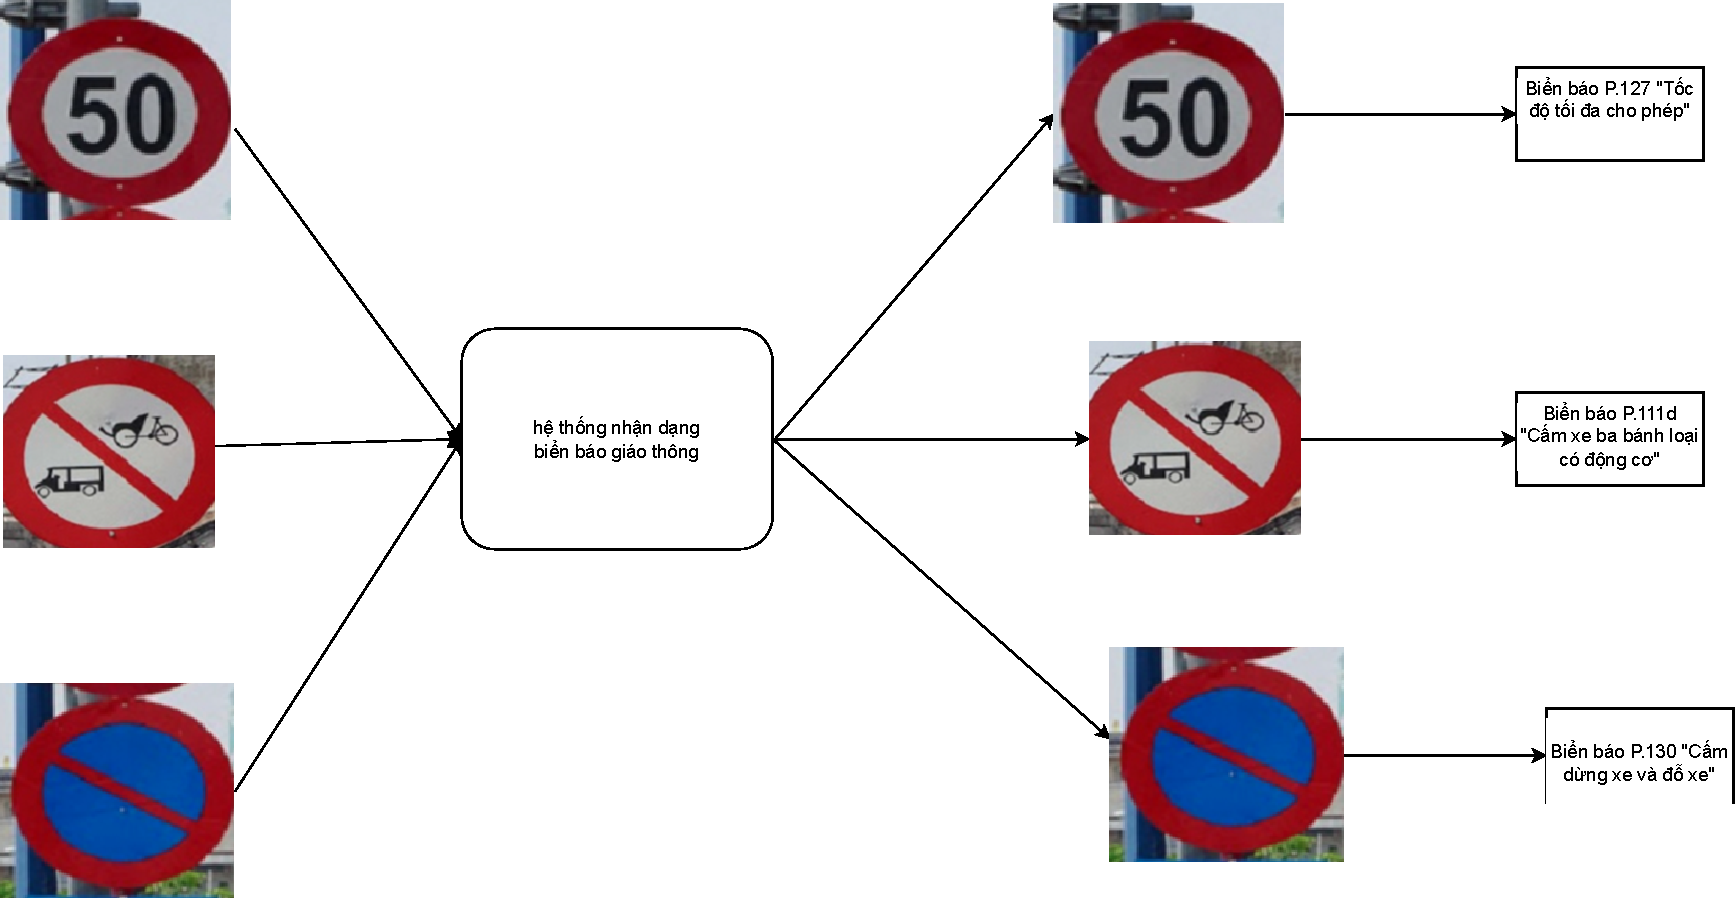
\includegraphics[width=\textwidth]{figures/anhnhandien.pdf}
\caption[Minh hoạ bài toán nhận diện biển báo giao thông]{Minh hoạ bài toán nhận diện biển báo giao thông}
\label{fig:traffic_sign_tasks}
\end{figure}

\subsection{Mô tả bằng toán học}
Gọi ảnh ở thời điểm $t$ là $I_t\in\{0,\ldots,255\}^{H_t\times W_t\times3}$, trong đó $H_t,W_t$ là chiều cao và chiều rộng. Tập nhãn của mô hình là $\mathcal{C}=\{0,1,\ldots,26\}$, theo tệp cấu hình lớp của dự án.

Kết quả tại thời điểm $t$ được mô tả bởi tập:
\begin{equation}
 \widehat{\mathcal{Y}}_t=
 \left\{(b_{tj},c_{tj},s_{tj},k_{tj},o_{tj})\right\}_{j=1}^{n_t}.
 \label{eq:output_problem}
\end{equation}
Trong đó $n_t$ là số biển được giữ lại; $b_{tj}$ là khung bao; $c_{tj}\in\mathcal{C}$ là lớp; $s_{tj}\in[0,1]$ là điểm tin cậy; $k_{tj}$ là mã theo vết hoặc giá trị rỗng với ảnh tĩnh. Thành phần $o_{tj}$ chứa thông tin bổ sung: chữ trên biển chính, chữ trên biển phụ, giá trị số, đơn vị và trạng thái đọc.

Gọi $\Sigma$ là bảng ký tự gồm chữ tiếng Việt, chữ số và các dấu cần đọc; $\Sigma^*$ là tập các chuỗi hữu hạn tạo từ bảng đó. Chuỗi chữ thuộc $\Sigma^*\cup\{\bot\}$; giá trị số thuộc $\mathbb{R}\cup\{\bot\}$ và đi kèm đơn vị khi đọc được. Ký hiệu $\bot$ biểu thị chưa có kết quả hoặc không áp dụng; nó khác với giá trị số 0. Một đối tượng có thể đã có lớp và vị trí nhưng nội dung chữ vẫn là $\bot$.

Khung bao dùng toạ độ điểm ảnh của ảnh gốc, có gốc ở góc trên bên trái:
\begin{equation}
 \begin{aligned}
 b_{tj}&=(x_{tj}^{\min},y_{tj}^{\min},x_{tj}^{\max},y_{tj}^{\max}),\\
 0&\le x_{tj}^{\min}<x_{tj}^{\max}\le W_t,\\
 0&\le y_{tj}^{\min}<y_{tj}^{\max}\le H_t.
 \end{aligned}
 \label{eq:box_problem}
\end{equation}
Toạ độ từ ảnh đã đổi kích thước được quy đổi về ảnh gốc trước khi cắt vùng hoặc hiển thị. Với ảnh không có biển phù hợp, tập kết quả là rỗng. Kích thước của một biển được đo bằng cạnh tương đương $\sqrt{wh}$ của khung bao (đơn vị điểm ảnh); các nhóm kích thước $<16$, $16$--$32$, $32$--$64$ và $\ge64$~px được dùng xuyên suốt báo cáo.

Gọi $\mathcal{S}_{t-1}$ là trạng thái lưu từ các khung hình trước, gồm các đối tượng đang theo vết và kết quả chữ đã có. Ánh xạ xử lý được viết:
\begin{equation}
 (\widehat{\mathcal{Y}}_t,\mathcal{S}_t)
 =F_{\theta,\psi,\omega}(I_t,\mathcal{S}_{t-1}).
 \label{eq:system_problem}
\end{equation}
Ở đây $\theta$ là tham số mô hình phát hiện, $\psi$ là tham số bộ xác minh và $\omega$ là tham số bộ nhận dạng chữ. Với ảnh tĩnh, trạng thái ban đầu rỗng. Ba bộ tham số được học hoặc nạp riêng; biểu thức~\eqref{eq:system_problem} mô tả quan hệ đầu vào--đầu ra, không phải một hàm mất mát chung để huấn luyện toàn hệ thống.

\subsection{Phạm vi và giới hạn xử lý}
Bộ nhãn có 27 lớp, gồm 26 lớp được giữ riêng và một lớp ``Biển báo khác''. Sáu lớp có ít hơn 60 cụm cảnh độc lập được gộp vào lớp này theo quyết định thiết kế của nhóm~\cite{utci_nhanlop}; lớp gộp không phải bộ nhận diện mọi biển ngoài dữ liệu và hệ thống không trả tên chi tiết của từng biển trong đó.

Chức năng đọc số áp dụng cho biển giới hạn tốc độ (km/h) và giới hạn chiều cao (m). Lớp giới hạn trọng lượng đã được gộp vào ``Biển báo khác'', nên đọc tải trọng không thuộc phạm vi. Biển phụ chưa là một lớp phát hiện độc lập; vùng biển phụ được tìm bằng xử lý ảnh phía dưới biển chính.

Bộ dữ liệu được giữ cố định ở phiên bản v1: nhóm không bổ sung ảnh và không gán thêm nhãn. Vì vậy, không có nhãn chữ để đo định lượng khả năng đọc chữ, và không có tập kiểm thử ngoài phân phối. Đề tài không giải quyết nhận diện đèn tín hiệu, vạch kẻ đường hoặc điều khiển phương tiện.

\subsection{Khó khăn trong nhận diện}
Biển báo có màu, hình dạng và ký hiệu tương đối rõ, nhưng ảnh thu nhận thay đổi theo khoảng cách, góc nhìn và điều kiện ghi hình. Biển ở xa chiếm ít điểm ảnh; trong dữ liệu của đề tài, 53,7\% số biển có cạnh dưới 32~px (Mục~\ref{sec:data_eda}). Góc nghiêng làm thay đổi hình dạng; mưa, bóng đổ, rung máy hoặc che khuất làm mất nét. Các bộ dữ liệu quy mô lớn cũng cho thấy biển nhỏ là thách thức chính~\cite{zhu2016tt100k,ertler2020mapillary}.

Các lớp biển có thể chỉ khác nhau ở một ký hiệu hoặc chữ số nhỏ. Nền đường phố lại chứa logo, quảng cáo, áo hoặc xe cùng màu với biển. Dữ liệu mất cân bằng khiến mô hình học lớp phổ biến tốt hơn lớp ít mẫu; vì vậy chỉ số trung bình cần được xem cùng kết quả theo lớp và theo kích thước.

\subsection{Các hướng tiếp cận}
Hướng dựa trên màu và hình dạng chọn các vùng đỏ, xanh hoặc vàng, làm sạch mặt nạ rồi kiểm tra đường bao gần tròn, tam giác hay chữ nhật~\cite{escalera1997road,maldonado2007svm}. Các bước dễ quan sát và giải thích, nhưng ngưỡng màu thay đổi theo ánh sáng, còn hình dạng bị ảnh hưởng bởi góc nhìn và che khuất. Hướng đặc trưng thủ công kết hợp học máy đưa màu, hình dạng hoặc HOG vào bộ phân loại; khi đầu vào là cả cảnh đường phố, vẫn cần một bước tạo vùng ứng viên.

Hướng học sâu học biểu diễn trực tiếp từ dữ liệu; mạng phát hiện dự đoán cả vị trí và lớp. Trong một hệ thống kết hợp, mỗi thành phần đảm nhiệm một nhiệm vụ: tăng cường ảnh, tìm biển, xác minh, đọc chữ, tổng hợp theo thời gian. Mỗi khâu thêm vào cần được đo đóng góp riêng, vì thêm bước xử lý làm tăng thời gian và có thể phát sinh lỗi mới. Đây là nguyên tắc chính của phần thực nghiệm.

\section{Dữ liệu và cách chuẩn bị}
\label{sec:data}

\subsection{Nguồn dữ liệu và nhãn}
Dự án sử dụng bộ dữ liệu biển báo Việt Nam \textit{merge\_Real-time Viet Nam Traffic Dtctn 2} trên Roboflow, giấy phép CC BY 4.0~\cite{roboflow_dataset,utci_data}. Bộ dữ liệu gộp từ nhiều nguồn, trong đó có ảnh đường phố của Zalo AI Challenge 2020~\cite{zalo2020tsd}. Nhãn ở định dạng YOLO: với tâm $(x_c,y_c)$, chiều rộng $w$, chiều cao $h$ trên ảnh $W\times H$, các giá trị lưu là $x_c/W$, $y_c/H$, $w/W$ và $h/H$. Nhãn gốc có 32 lớp; ánh xạ sang 27 lớp mô hình nằm trong danh mục lớp của dự án, kèm mã hiệu QCVN, nhóm biển và ý nghĩa.

\subsection{Kiểm tra, lọc và chia dữ liệu}
Quy trình chuẩn bị gồm năm bước (Hình~\ref{fig:data_flow}a):
\begin{enumerate}
 \item Kiểm tra toàn bộ 5\,453 ảnh và 13\,478 nhãn gốc: không có ảnh hỏng định dạng hay khung bao vượt biên; 12 ảnh lỗi nội dung và 55 ảnh còn biển chưa được gán nhãn bị loại (ghi danh sách cùng lý do).
 \item Tìm ảnh gần trùng bằng băm cảm nhận pHash $8\times8$~\cite{imagehash_phash}; hai ảnh có khoảng cách Hamming $\le6$ thuộc cùng một cụm. Kết quả có 3\,889 cụm cảnh.
 \item Gộp sáu lớp có dưới 60 cụm cảnh vào ``Biển báo khác'', còn 27 lớp.
 \item Chia lại theo cụm với tỉ lệ 70/15/15, phân tầng theo lớp và độ phân giải, hạt giống 42. Mọi ảnh của một cụm nằm trong cùng một tập, nên tập kiểm thử không chứa ảnh gần trùng với tập huấn luyện.
 \item Đóng gói thành phiên bản dữ liệu v1 kèm mã băm và báo cáo chia tập.
\end{enumerate}

\begin{figure}[H]
\centering
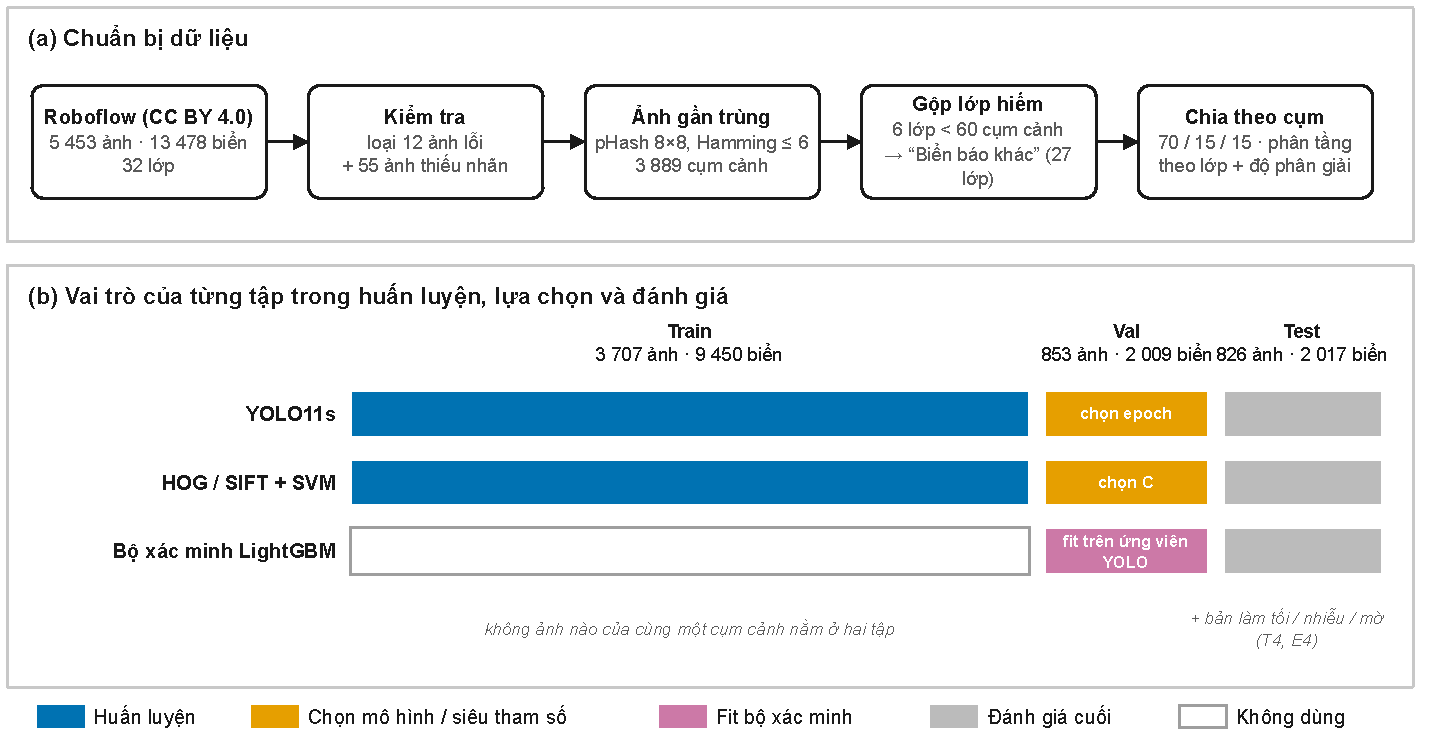
\includegraphics[width=\textwidth]{figures/Fig_du_lieu.pdf}
\caption[Chuẩn bị dữ liệu và vai trò của từng tập]{Chuẩn bị dữ liệu (a) và vai trò của từng tập đối với các mô hình (b)}
\label{fig:data_flow}
\fignote{Độ rộng thanh tỉ lệ với số ảnh (Val và Test được nới tối thiểu để đọc được nhãn).}
\end{figure}

Bảng~\ref{tab:split} cho số ảnh và số biển sau khi chia. Hình~\ref{fig:data_flow}b cho biết mỗi tập được dùng vào việc gì: tập huấn luyện để học tham số, tập xác thực để chọn epoch của YOLO, chọn tham số $C$ của SVM và học bộ xác minh; tập kiểm thử chỉ dùng cho đánh giá cuối và không tham gia bất kỳ lựa chọn nào.

\begin{table}[H]
\centering
\caption{Thống kê bộ dữ liệu sau khi chia theo cụm}
\label{tab:split}
\small
\begin{tabularx}{\textwidth}{|>{\raggedright\arraybackslash}X|>{\centering\arraybackslash}p{2.2cm}|>{\centering\arraybackslash}p{2.2cm}|>{\centering\arraybackslash}p{2.2cm}|>{\centering\arraybackslash}p{2.2cm}|}
\toprule
 & \textbf{Train} & \textbf{Val} & \textbf{Test} & \textbf{Tổng} \\
\midrule
Số ảnh & 3\,707 & 853 & 826 & 5\,386 \\ \hline
Số biển (khung bao) & 9\,450 & 2\,009 & 2\,017 & 13\,476 \\ \hline
Tỉ lệ ảnh (\%) & 68,8 & 15,8 & 15,3 & 100 \\
\bottomrule
\end{tabularx}
\tablenote{53 ảnh không có biển được giữ làm ảnh nền.}
\end{table}

\subsection{Phân tích khám phá dữ liệu}
\label{sec:data_eda}
Hình~\ref{fig:eda_size} và Hình~\ref{fig:eda_class} tóm tắt các đặc điểm ảnh hưởng trực tiếp đến thiết kế:
\begin{itemize}
 \item Biển rất nhỏ. Cạnh tương đương trung vị là 30~px; 18,3\% số biển nhỏ hơn 16~px và 53,7\% nhỏ hơn 32~px. Một số lớp có tới 38--48\% số biển dưới 16~px (Cấm đi ngược chiều, Phải đi vòng sang bên phải, Giới hạn chiều cao, Vạch sang đường cho người đi bộ).
 \item Bốn độ phân giải. $960\times540$ (2\,346 ảnh), $1622\times626$ (2\,213 ảnh, nguồn Zalo), $1920\times1080$ (798 ảnh) và $540\times960$ (29 ảnh). Ảnh $1622\times626$ có nhiều biển nhỏ ở xa.
 \item Mất cân bằng lớp. Nhiều nhất là Giới hạn tốc độ (1\,705 biển), ít nhất là Chỗ quay xe (76 biển), chênh 22 lần; trước khi gộp là 55 lần. Biển cấm chiếm 57\% số biển.
 \item Nhiều biển trên một ảnh. Trung bình 2,5 biển mỗi ảnh; 73 ảnh có từ 10 biển trở lên.
\end{itemize}

\begin{figure}[H]
\centering
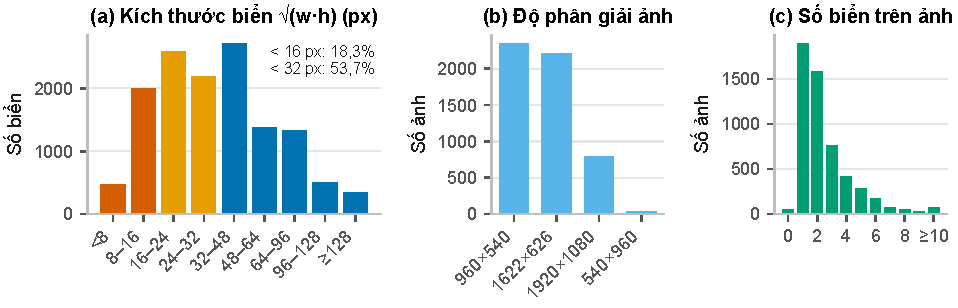
\includegraphics[width=\textwidth]{figures/ch2_eda_kich_thuoc.pdf}
\caption{Phân bố kích thước biển, độ phân giải ảnh và số biển trên mỗi ảnh}
\label{fig:eda_size}
\fignote{Cột đỏ: biển $<16$~px; cột cam: $16$--$32$~px.}
\end{figure}

\begin{figure}[H]
\centering
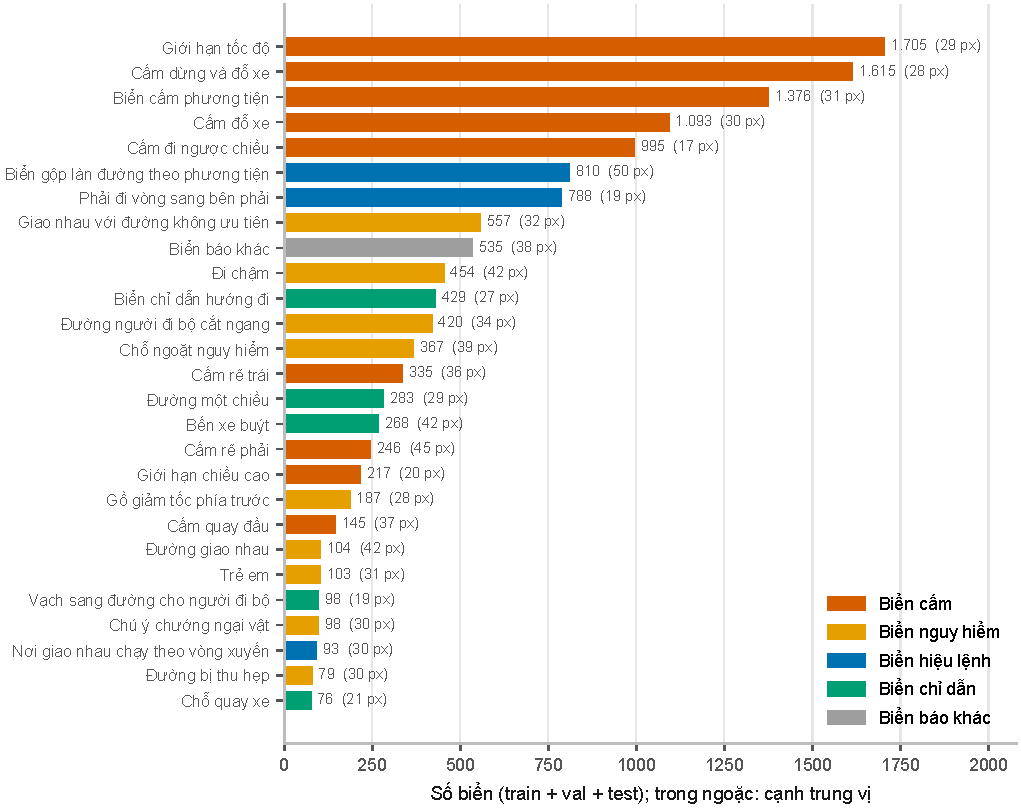
\includegraphics[width=.92\textwidth]{figures/ch2_eda_lop.pdf}
\caption{Số biển của 27 lớp theo nhóm biển; trong ngoặc là cạnh tương đương trung vị}
\label{fig:eda_class}
\end{figure}

\subsection{Dữ liệu chữ và video}
Nhãn lớp và khung bao không đủ để đo khả năng đọc nội dung: cần bản chép đúng của giá trị số và chữ, kể cả dấu tiếng Việt. Vì dữ liệu được đóng băng, đề tài không có nhãn chữ; khả năng đọc chữ chỉ được đánh giá định tính trên ảnh của tập kiểm thử. Video chỉ dùng để minh hoạ chức năng theo vết; ghép ảnh tĩnh thành video không hợp lệ cho việc đo độ ổn định nhãn vì cảnh thay đổi sau mỗi vài khung hình.

\section{Kiến trúc tổng thể}
\label{sec:architecture}

Hình~\ref{fig:system_pipeline} là kiến trúc của hệ thống chính, được dùng chung cho API ảnh, xử lý video nền và webcam~\cite{utci_thietke}. Mỗi khâu được gắn nhãn theo loại phương pháp: CV cho xử lý ảnh và đặc trưng thủ công, DL cho học sâu. Mỗi khâu có cờ bật/tắt trong tệp cấu hình để đo đóng góp riêng.

\begin{figure}[H]
\centering
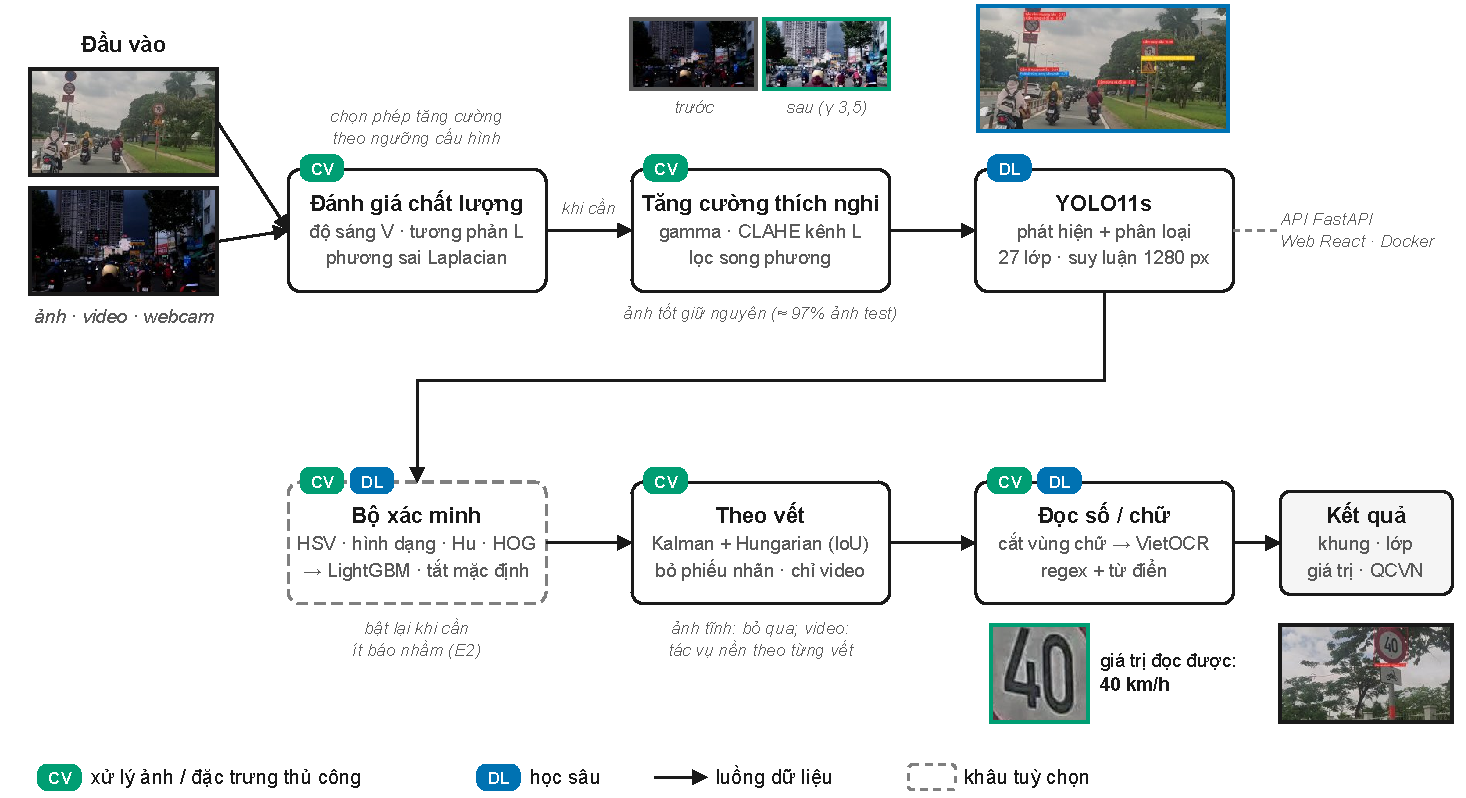
\includegraphics[width=\textwidth]{figures/Fig_pipeline_he_thong.pdf}
\caption[Kiến trúc hệ thống nhận diện biển báo]{Kiến trúc hệ thống nhận diện biển báo: đánh giá chất lượng và tăng cường thích nghi [CV] $\rightarrow$ YOLO11s [DL] $\rightarrow$ bộ xác minh (tuỳ chọn) $\rightarrow$ theo vết [CV] $\rightarrow$ đọc số, chữ [CV + DL]}
\label{fig:system_pipeline}
\fignote{Ảnh nhỏ là kết quả trung gian thật của hệ thống trên ảnh thuộc tập kiểm thử.}
\end{figure}

Luồng xử lý một khung hình gồm năm bước:
\begin{enumerate}
 \item Đánh giá chất lượng [CV]: đo độ sáng, tương phản và độ nét trên ảnh thu nhỏ; chỉ khi các chỉ báo vượt ngưỡng mới tăng cường. Ảnh tốt đi thẳng qua.
 \item Phát hiện và phân loại [DL]: YOLO11s trả khung bao, lớp và điểm tin cậy cho 27 lớp.
 \item Xác minh [CV + DL, tuỳ chọn]: LightGBM trên đặc trưng thủ công và ngữ cảnh YOLO đánh giá lại từng phát hiện. Khâu này tắt mặc định dựa trên kết quả thử nghiệm (Mục~\ref{sec:t1}).
 \item Theo vết [CV]: với video, ghép phát hiện qua các khung hình bằng Kalman và Hungarian, bỏ phiếu nhãn theo vết.
 \item Đọc số, chữ [CV + DL]: cắt vùng chữ bằng xử lý ảnh, đọc bằng VietOCR, kiểm tra bằng biểu thức chính quy và từ điển; ghép với thông tin QCVN của lớp để trả kết quả.
\end{enumerate}
Với ảnh tĩnh, các khâu chạy tuần tự. Với video, xác minh và đọc chữ chạy nền theo từng vết (khi vết mới xuất hiện hoặc sau mỗi 10 khung hình), nên không chặn luồng phát hiện.

Song song với hệ thống chính, nhóm xây dựng một hệ thống đối chứng chỉ dùng thị giác máy tính truyền thống (Mục~\ref{sec:cv_pipeline}). Hệ thống đối chứng không dùng trong sản phẩm; nó dùng để so sánh hai phương pháp trên cùng ảnh và cùng tập kiểm thử (Chương~\ref{chap:chuong3}).

\section{Phương pháp học sâu}
\label{sec:deep}

\subsection{Mô hình phát hiện YOLO11s}
Nhóm chọn YOLO11 của Ultralytics~\cite{ultralytics_yolo11,khanam2024yolo11}, biến thể nhỏ YOLO11s, khởi tạo từ trọng số học trên COCO~\cite{lin2014coco} rồi tinh chỉnh toàn bộ mạng trên tập huấn luyện. Một mô hình đảm nhiệm cả tìm vị trí và phân loại, nên hệ thống không cần mạng phân loại biển riêng. Bảng~\ref{tab:ch2_detector_config} là cấu hình dùng cho lần huấn luyện được chọn~\cite{utci_cauhinh}.

\begin{table}[H]
\centering
\caption{Cấu hình huấn luyện và suy luận của YOLO11s}
\label{tab:ch2_detector_config}
\small
\begin{tabularx}{\textwidth}{|>{\raggedright\arraybackslash}p{3.6cm}|>{\raggedright\arraybackslash}X|}
\toprule
\textbf{Thành phần} & \textbf{Giá trị} \\
\midrule
Trọng số khởi tạo & YOLO11s đã huấn luyện trước trên COCO \\ \hline
Kích thước ảnh huấn luyện & 960 px (cạnh dài), giữ tỉ lệ và đệm theo thư viện \\ \hline
Số epoch, kích thước lô & 80 epoch; 8 ảnh mỗi lô \\ \hline
Tối ưu & AdamW, tốc độ học ban đầu $0{,}001$, lịch cosine, 3 epoch khởi động \\ \hline
Tăng cường dữ liệu & Mặc định của thư viện; tắt lật ngang (tránh đổi nghĩa biển trái--phải); tắt mosaic ở 15 epoch cuối \\ \hline
Chọn trọng số & Epoch có mAP@50:95 cao nhất trên tập xác thực \\ \hline
Môi trường & Google Colab, Tesla T4; Ultralytics 8.4.183; 2 giờ 52 phút \\ \hline
Suy luận & 1280 px (chọn theo thí nghiệm T3), ngưỡng điểm $0{,}25$, NMS với IoU $0{,}5$, FP16 trên GPU \\
\bottomrule
\end{tabularx}
\end{table}

Mô hình được huấn luyện ở 960 px nhưng suy luận ở 1280 px. Phóng to ảnh khi suy luận làm biển nhỏ chiếm nhiều điểm ảnh hơn trên bản đồ đặc trưng mà không cần huấn luyện lại; thí nghiệm T3 (Mục~\ref{sec:t3}) cho thấy cách này tăng recall biển nhỏ mà không giảm precision. Hệ thống cũng có tuỳ chọn cắt ô $640\times640$ chồng lấn theo ý tưởng SAHI~\cite{akyon2022sahi} cho ảnh độ phân giải cao.

\subsection{Đọc chữ và giá trị số}
Nhận dạng ký tự quang học (OCR) gồm bước tìm vùng chữ và bước nhận dạng nội dung (Hình~\ref{fig:ocr_basic})~\cite{paddleocr_overview}. Hệ thống tách hai bước theo hai loại phương pháp: vùng chữ được cắt bằng xử lý ảnh [CV], nội dung được đọc bằng VietOCR với cấu hình VGG-Transformer (trích đặc trưng VGG, giải mã Transformer) [DL]~\cite{vietocr_repo}.

\begin{figure}[H]
\centering
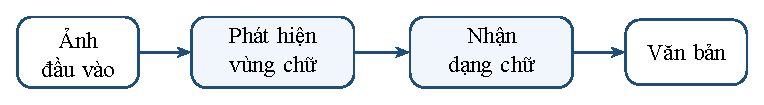
\includegraphics[width=.9\textwidth]{figures/fig_1_6_ocr.pdf}
\caption[Kiến trúc OCR cơ bản]{Kiến trúc OCR cơ bản: phát hiện vùng chữ và nhận dạng nội dung}
\label{fig:ocr_basic}
\end{figure}

\begin{itemize}
 \item Biển có giá trị số (tốc độ, chiều cao): cắt đĩa phía trong viền đỏ (78\% đường kính), phóng to 3 lần, yêu cầu chiều cao vùng tối thiểu 40~px.
 \item Dòng chữ và biển phụ: tìm tấm chữ nhật sáng phía dưới biển chính (vùng tìm cao 1,2 lần biển chính), tách dòng bằng chiếu histogram theo hàng, tăng tương phản bằng CLAHE và chỉnh nghiêng trước khi đọc.
 \item Hậu xử lý: biểu thức chính quy tách số và đơn vị; giá trị tốc độ phải thuộc danh sách hợp lệ (5--120 km/h), chiều cao trong khoảng 1,5--6 m; chữ được so với từ điển bằng độ tương đồng chuỗi (ngưỡng 80/100). Dòng có độ tin cậy VietOCR dưới 0,75 bị bỏ.
\end{itemize}
Chuỗi gốc và chuỗi sau xử lý đều được lưu. Quy tắc sửa không được ``đoán'': nếu ảnh chưa phân biệt được 50 và 60, danh sách giá trị hợp lệ không đủ căn cứ để chọn, và kết quả để trống. Với video, vùng đọc được chọn từ khung hình có tích diện tích và độ nét lớn nhất của vết.

\section{Phương pháp thị giác máy tính truyền thống}
\label{sec:classic}

\subsection{Đánh giá chất lượng và tăng cường ảnh thích nghi}
\label{sec:enhance}
Ảnh được thu nhỏ về chiều rộng 320 px rồi đo ba chỉ báo: độ sáng trung bình $\mu_V$ của kênh V (HSV), độ lệch chuẩn $\sigma_L$ của kênh L (Lab) và phương sai đáp ứng Laplacian $\sigma^2_{\nabla^2}$ trên ảnh xám. Tập phép tăng cường được chọn theo quy tắc:
\begin{equation}
 \mathcal{O}=
 \begin{cases}
  \{\text{gamma},\text{CLAHE}\} & \text{nếu } \mu_V<0{,}30,\\
  \{\text{CLAHE}\} & \text{nếu } \sigma_L<0{,}13,\\
  \{\text{lọc song phương}\} & \text{nếu } \sigma^2_{\nabla^2}>4000,
 \end{cases}
 \label{eq:enhance_rule}
\end{equation}
(lấy hợp của các điều kiện thoả mãn). Các ngưỡng được chọn từ thống kê dữ liệu ở Sprint 1, trước khi có tập kiểm thử của các thí nghiệm; ảnh không thoả điều kiện nào được giữ nguyên.

Gamma tự động đưa độ sáng trung bình về $0{,}5$:
\begin{equation}
 \gamma=\operatorname{clip}\!\left(\frac{\ln\mu_V}{\ln0{,}5},\,0{,}4,\,3{,}0\right),\qquad
 I'(x,y)=255\left(\frac{I(x,y)}{255}\right)^{1/\gamma}.
 \label{eq:gamma}
\end{equation}
Với ảnh tối ($\mu_V<0{,}5$) ta có $\gamma>1$, nên số mũ $1/\gamma<1$ làm sáng ảnh. CLAHE~\cite{zuiderveld1994clahe} được áp trên kênh L của không gian Lab (giới hạn tương phản 2,0, lưới $8\times8$), tăng tương phản cục bộ mà không làm lệch màu đỏ, xanh, vàng của biển. Lọc song phương~\cite{tomasi1998bilateral} (đường kính 5, $\sigma_{\text{màu}}=\sigma_{\text{không gian}}=50$) giảm nhiễu nhưng giữ biên. Thiết kế ``chỉ tăng cường khi cần'' xuất phát từ quan sát rằng áp dụng mọi phép cho mọi ảnh có thể làm hại ảnh tốt hoặc ảnh nhiễu; thí nghiệm T4 (Mục~\ref{sec:t4}) kiểm chứng điều này.

\subsection{Pipeline đối chứng: màu, hình dạng, HOG và SVM}
\label{sec:cv_pipeline}
Pipeline đối chứng giải toàn bộ bài toán phát hiện và phân loại mà không dùng mạng nơ-ron (Hình~\ref{fig:cv_pipeline}). Nó kế thừa hướng màu--hình dạng của các công trình kinh điển~\cite{escalera1997road,maldonado2007svm} và đặc trưng HOG~\cite{dalal2005hog}.

\begin{figure}[H]
\centering
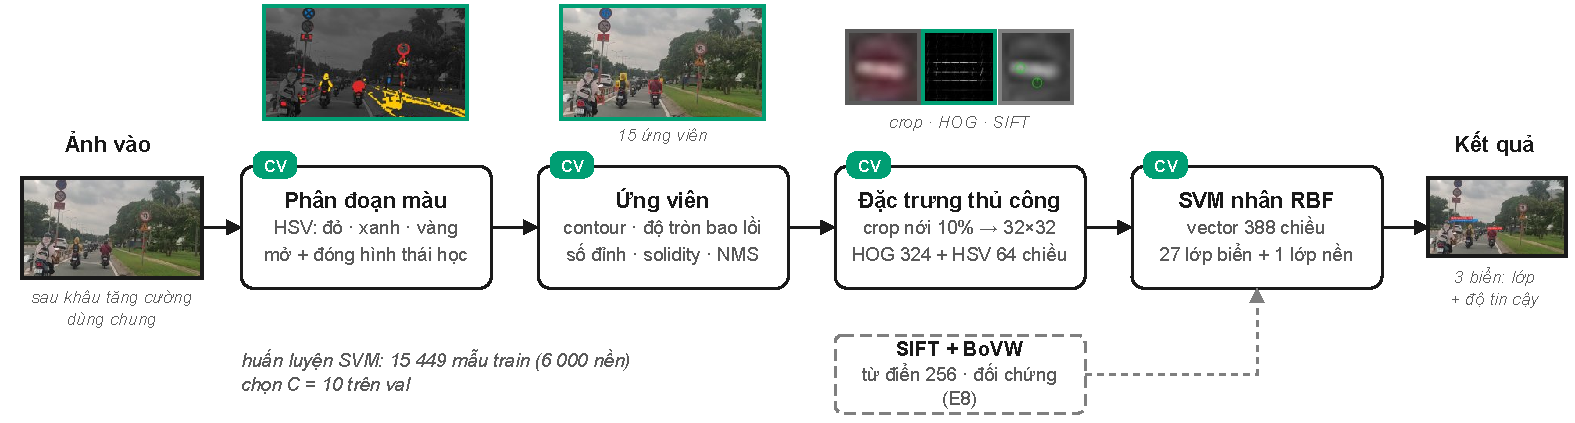
\includegraphics[width=\textwidth]{figures/Fig_pipeline_cv.pdf}
\caption[Pipeline CV truyền thống đối chứng]{Pipeline CV truyền thống đối chứng: phân đoạn màu HSV $\rightarrow$ ứng viên theo hình dạng $\rightarrow$ HOG + histogram HSV $\rightarrow$ SVM có lớp nền}
\label{fig:cv_pipeline}
\end{figure}

\paragraph{Phân đoạn màu.} Ảnh được chuyển sang HSV và lấy ngưỡng theo ba màu quy chuẩn: đỏ (hai dải $H\in[0,10]\cup[160,179]$ vì sắc đỏ nằm ở hai đầu vòng màu, $S\ge70$, $V\ge50$), xanh ($H\in[95,130]$) và vàng ($H\in[15,35]$). Mỗi mặt nạ được mở rồi đóng bằng phần tử cấu trúc $3\times3$ để bỏ điểm nhiễu và nối viền bị đứt.

\paragraph{Ứng viên theo hình dạng.} Với mỗi đường bao ngoài có diện tích từ 60~px$^2$ đến 25\% ảnh, hệ thống tính tỉ lệ khung $a=w/h$, số đỉnh $k$ sau xấp xỉ đa giác (sai số $0{,}04$ chu vi), độ đặc $\rho=A/A_{\text{bao lồi}}$ và độ tròn của bao lồi
\begin{equation}
 C_{\text{hull}}=\frac{4\pi A_{\text{hull}}}{P_{\text{hull}}^2}.
 \label{eq:hull_circularity}
\end{equation}
Viền đỏ của biển cấm là một vòng rỗng nên độ tròn của chính đường bao thấp; dùng bao lồi khắc phục điều này. Vùng được nhận là \textit{tròn} nếu $0{,}6\le a\le1{,}6$ và $C_{\text{hull}}\ge0{,}75$; \textit{tam giác} nếu màu đỏ hoặc vàng, $k=3$, $0{,}7\le a\le1{,}5$, $\rho>0{,}6$; \textit{chữ nhật} nếu màu xanh, $4\le k\le6$, $0{,}5\le a\le3$, $\rho>0{,}8$. Các ứng viên trùng nhau được loại bằng NMS (IoU $0{,}3$) và loại mảnh màu nằm trong một biển lớn hơn.

\paragraph{Đặc trưng thủ công.} Mỗi ứng viên được cắt nới 10\% mỗi phía và đưa về $32\times32$. HOG trên ảnh xám dùng 9 hướng, ô $8\times8$, khối $2\times2$, cho vector 324 chiều mô tả ký hiệu bên trong biển. Histogram HSV $16\times4$ (16 mức sắc độ, 4 mức bão hoà) chuẩn hoá tổng bằng 1, cho 64 chiều mô tả màu. Vector ghép có 388 chiều. Hai loại đặc trưng bổ sung cho nhau: HOG trên ảnh xám bỏ qua màu, trong khi màu lại là thông tin quy chuẩn phân biệt biển cấm, nguy hiểm và hiệu lệnh.

\paragraph{Phân loại bằng SVM.} SVM nhân RBF~\cite{cortes1995svm} sau bước chuẩn hoá đặc trưng phân loại 28 lớp: 27 lớp biển và một lớp \textit{nền}. Mẫu nền là các ứng viên màu--hình dạng trên ảnh huấn luyện không trùng biển thật nào (IoU $<0{,}1$); nhờ lớp này, SVM loại được vùng màu giả như áo, xe, mái tôn. Tập huấn luyện có 15\,449 mẫu (6\,000 nền), trọng số lớp cân bằng; $C\in\{1,10\}$ được chọn trên tập xác thực (3\,509 mẫu), kết quả $C=10$. Ứng viên có xác suất dưới 0,30 không được hiển thị. Hình~\ref{fig:cv_steps} minh hoạ các bước trên một ảnh của tập kiểm thử.

\begin{figure}[H]
\centering
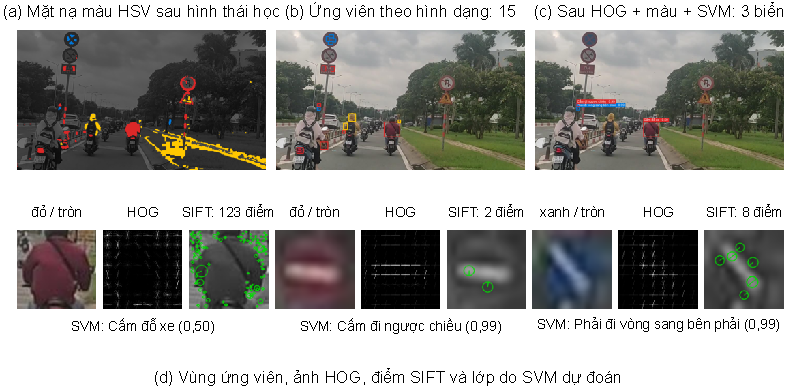
\includegraphics[width=\textwidth]{figures/ch2_cv_buoc.pdf}
\caption{Các bước của pipeline CV truyền thống trên một ảnh của tập kiểm thử}
\label{fig:cv_steps}
\fignote{Vùng thứ nhất ở (d) là áo đỏ bị nhận nhầm thành ``Cấm đỗ xe'' với xác suất 0,50 --- một dạng báo động giả điển hình của hướng màu--hình dạng.}
\end{figure}

\paragraph{SIFT kết hợp túi từ thị giác (đối chứng âm).} Để kiểm chứng việc chọn HOG, nhóm cài thêm SIFT~\cite{lowe2004sift} trên vùng biển phóng về $64\times64$, lượng tử hoá thành từ điển 256 từ bằng k-means (MiniBatch) và biểu diễn mỗi vùng bằng histogram từ~\cite{csurka2004bovw}, sau đó dùng cùng SVM. Biển báo có ít kết cấu, nên dự kiến SIFT sẽ kém HOG; thí nghiệm E8 kiểm chứng dự kiến này.

\subsection{Bộ xác minh}
\label{sec:verifier}
Bộ xác minh đánh giá lại một phát hiện của YOLO bằng đặc trưng thủ công của vùng đó. Với vùng $b_j$, lớp $c_j$ và điểm $s_j^{\mathrm{det}}$:
\begin{equation}
 z_j=\varphi(I,b_j,c_j,s_j^{\mathrm{det}}),\qquad
 q_j=g_{\psi}(z_j).
 \label{eq:verifier_problem}
\end{equation}
Hàm $\varphi$ trích vector $z_j$ gồm ngữ cảnh YOLO (điểm, lớp, kích thước, vị trí), tỉ lệ màu HSV, đặc trưng hình học, bảy moment Hu~\cite{hu1962moments} và HOG giảm chiều bằng PCA (16 thành phần); $g_\psi$ là LightGBM~\cite{ke2017lightgbm} (400 cây, tốc độ học $0{,}05$, 31 lá, cân bằng lớp) kèm hiệu chỉnh xác suất isotonic. Nhãn huấn luyện lấy từ các phát hiện của YOLO trên tập xác thực với ngưỡng thấp $0{,}10$: phát hiện đúng lớp và có IoU $\ge0{,}5$ với một biển thật là mẫu dương, còn lại là mẫu âm. Ý tưởng này theo hướng ``theo vết rồi lọc bằng mô hình phân biệt riêng'' của Šegvić và cộng sự~\cite{segvic2014temporal}. Thí nghiệm T1 cho thấy bộ xác minh không vượt được điểm tin cậy của chính YOLO, nên khâu này được tắt mặc định (Mục~\ref{sec:t1}).

\subsection{Theo vết và tổng hợp nhãn}
Theo vết liên kết các phát hiện của cùng một biển qua nhiều khung hình theo cách của SORT~\cite{bewley2016sort}. Bộ lọc Kalman~\cite{kalman1960filter} ước lượng trạng thái 8 chiều gồm tâm $(c_x,c_y)$, kích thước $(w,h)$ của khung và vận tốc biến đổi của bốn đại lượng này trên ảnh; bước dự đoán ước lượng vị trí ở khung tiếp theo, bước cập nhật kết hợp dự đoán với phát hiện mới. Phát hiện mới được ghép với vết đang có bằng thuật toán Hungarian~\cite{kuhn1955hungarian} sao cho tổng IoU giữa khung dự đoán và khung phát hiện lớn nhất; cặp có IoU dưới $0{,}3$ bị loại.

Vết được xác nhận sau 3 lần quan sát và bị xoá sau 15 khung hình không xuất hiện lại. Nhãn hiển thị của vết là lớp có tổng điểm lớn nhất trong cửa sổ 10 quan sát gần nhất, giúp giảm hiện tượng nhãn nhảy giữa các khung do mờ hoặc che khuất. Cửa sổ dài làm nhãn ổn định hơn nhưng chậm sửa một nhãn sai. Các đại lượng của bộ lọc mô tả chuyển động biểu kiến trên ảnh, không phải tốc độ hay khoảng cách vật lý của biển.

\section{Tổ chức huấn luyện và đánh giá}
\label{sec:protocol}

\subsection{Huấn luyện riêng từng mô hình}
Bốn mô hình được huấn luyện riêng với dữ liệu và mục tiêu khác nhau (Hình~\ref{fig:data_flow}b): YOLO11s trên ảnh huấn luyện; SVM của pipeline đối chứng trên vùng cắt từ ảnh huấn luyện; bộ xác minh trên phát hiện của YOLO ở tập xác thực; VietOCR dùng trọng số huấn luyện trước, không tinh chỉnh. Mỗi lần huấn luyện và mỗi lần đánh giá được ghi vào sổ đăng ký thí nghiệm gồm mã thí nghiệm, commit, cấu hình, môi trường và kết quả, để mọi con số trong Chương~\ref{chap:chuong3} truy được về một lần chạy cụ thể.

\subsection{Các chỉ số đánh giá phát hiện biển báo}
\label{sec:detection_metrics}
Độ giao trên hợp (IoU) đo mức chồng lấn giữa khung dự đoán $B_p$ và khung đúng $B_g$:
\begin{equation}
 \operatorname{IoU}(B_p,B_g)=\frac{|B_p\cap B_g|}{|B_p\cup B_g|}.
 \label{eq:iou}
\end{equation}
Tại một ngưỡng điểm và ngưỡng IoU, dự đoán đúng lớp và khớp với một nhãn thật chưa ghép là phát hiện đúng (TP); dự đoán sai lớp, không khớp hoặc trùng lặp là phát hiện sai (FP); biển thật chưa được phát hiện là bỏ sót (FN):
\begin{equation}
 \operatorname{P}=\frac{TP}{TP+FP},\qquad
 \operatorname{R}=\frac{TP}{TP+FN},\qquad
 F_1=\frac{2\,\mathrm{P}\,\mathrm{R}}{\mathrm{P}+\mathrm{R}}.
 \label{eq:precision_recall}
\end{equation}
Thay đổi ngưỡng điểm tạo đường precision--recall; AP tóm tắt đường này cho một lớp, mAP lấy trung bình giữa $C$ lớp~\cite{tailieu_bai9}:
\begin{equation}
 \operatorname{mAP}_{\tau}=\frac{1}{C}\sum_{c=1}^{C}AP_{c,\tau},\qquad
 \operatorname{mAP}_{50:95}=\frac{1}{10}\sum_{j=0}^{9}\operatorname{mAP}_{0.50+0.05j}.
 \label{eq:map}
\end{equation}
mAP@50 dùng ngưỡng IoU $0{,}5$; mAP@50:95 xét các ngưỡng từ $0{,}5$ đến $0{,}95$ nên đòi hỏi khung khớp chặt hơn~\cite{coco_evaluation,ultralytics_metrics}.

\subsection{Giao thức đánh giá}
Để kết quả phản ánh đúng hệ thống khi chạy thật và so sánh được giữa các cấu hình, nhóm cố định giao thức sau:
\begin{itemize}
 \item Điểm vận hành. Chỉ số chính là P, R, $F_1$ tại ngưỡng hiển thị của hệ thống (điểm $0{,}25$), đúng lớp và IoU $\ge0{,}5$. Precision ở ngưỡng tối ưu theo $F_1$ do thư viện báo cáo không phải điều người dùng nhìn thấy. Ma trận nhầm lẫn mặc định của Ultralytics~8.4 ghép cả dự đoán điểm $0{,}001$ nên không được dùng làm bằng chứng.
 \item Theo kích thước và theo lớp. Recall được tính riêng cho bốn nhóm kích thước và cho từng lớp, vì giá trị trung bình che lấp điểm yếu ở biển nhỏ và lớp hiếm.
 \item Khoảng tin cậy. CI 95\% của chỉ số toàn tập được ước lượng bằng bootstrap theo ảnh~\cite{efron1993bootstrap} (500--2\,000 lần lấy mẫu lặp; ghép cặp khi so hai cấu hình trên cùng ảnh); CI của tỉ lệ theo lớp dùng khoảng Wilson~\cite{wilson1927}. Hai cấu hình chỉ được coi là khác nhau khi CI của hiệu không chứa 0.
 \item Mức tương đồng với tập huấn luyện. Ảnh kiểm thử được chia ba nhóm theo khoảng cách pHash tới ảnh huấn luyện gần nhất ($\le10$, 11--14, $\ge15$ bit). Nhóm ``khác train'' cho ước lượng gần hơn với ảnh mới, thay cho tập ngoài phân phối mà đề tài không có.
 \item Ảnh xấu giả lập. Ảnh tối: $I'=255\,(I/255)^{\gamma}$ với $\gamma=2{,}5$ hoặc $3{,}5$; nhiễu Gauss $\sigma=15$; mờ chuyển động ngang với nhân 9~px.
 \item Tốc độ. Ghi rõ phần cứng, kích thước ảnh và các khâu được tính thời gian.
\end{itemize}

\subsection{Các thí nghiệm}
Bảng~\ref{tab:experiments} liệt kê các thí nghiệm, câu hỏi mỗi thí nghiệm trả lời và mục trình bày kết quả.

\begin{table}[H]
\centering
\caption{Danh sách thí nghiệm}
\label{tab:experiments}
\small
\begin{tabularx}{\textwidth}{|>{\centering\arraybackslash}p{1.1cm}|>{\raggedright\arraybackslash}X|>{\raggedright\arraybackslash}p{4.4cm}|>{\centering\arraybackslash}p{1.5cm}|}
\toprule
\textbf{Mã} & \textbf{Câu hỏi} & \textbf{Thiết kế} & \textbf{Mục} \\
\midrule
S1 & YOLO11s học tốt đến đâu trên dữ liệu cùng nguồn? & Huấn luyện 960 px; mAP, CI bootstrap, theo lớp, kích thước, tương đồng & \ref{sec:baseline} \\ \hline
T0, T1 & Đặc trưng thủ công có giúp loại phát hiện sai của YOLO? & Ablation tập đặc trưng của bộ xác minh; P ở cùng recall & \ref{sec:t1} \\ \hline
T3 & Tăng recall biển nhỏ mà không huấn luyện lại? & Suy luận 960 / 1280 / cắt ô 640 & \ref{sec:t3} \\ \hline
T4, E4 & Tăng cường thích nghi có giúp khi ảnh xấu? & Ảnh tối, nhiễu, mờ; không xử lý / thích nghi / luôn áp & \ref{sec:t4} \\ \hline
E8 & Đặc trưng thủ công + SVM so với YOLO ở phân loại? & Cùng 2\,017 biển; theo kích thước; ghép cặp & \ref{sec:e8} \\ \hline
E1, E2 & Hệ thống mặc định đạt bao nhiêu; mỗi khâu đóng góp gì? & Cấu hình mặc định; ablation bật từng khâu & \ref{sec:e1} \\
\bottomrule
\end{tabularx}
\end{table}

\subsection{Đánh giá đọc chữ, tốc độ và độ ổn định}
Khả năng đọc chữ nên được đo bằng tỉ lệ lỗi ký tự $\operatorname{CER}=(S+D+I)/N$ và tỉ lệ khớp hoàn toàn~\cite{torchmetrics_cer}, trong đó $S,D,I$ là số phép thay, xoá, chèn và $N$ là độ dài chuỗi tham chiếu. Do không có nhãn chữ, đề tài chỉ đánh giá định tính. Số khung hình mỗi giây $\mathrm{FPS}=n/T$ và độ trễ từ lúc nhận ảnh đến lúc có kết quả được đo riêng cho khâu phát hiện, cho API ảnh và cho luồng WebSocket. Với video, độ ổn định nhãn được định nghĩa là tỉ lệ khung hình mà nhãn hiển thị của cùng một vết bị đổi; công cụ đo đã có nhưng chưa có video đường phố thật để đo.
